% Generated by code/needham.py -- do not edit by hand.
\definecolor{qocA}{rgb}{0.00,0.45,0.70}
\definecolor{qocB}{rgb}{0.90,0.60,0.00}
\definecolor{qocC}{rgb}{0.00,0.62,0.45}
\definecolor{qocD}{rgb}{0.80,0.40,0.00}
\definecolor{qocE}{rgb}{0.80,0.60,0.70}
\definecolor{qocF}{rgb}{0.35,0.70,0.90}
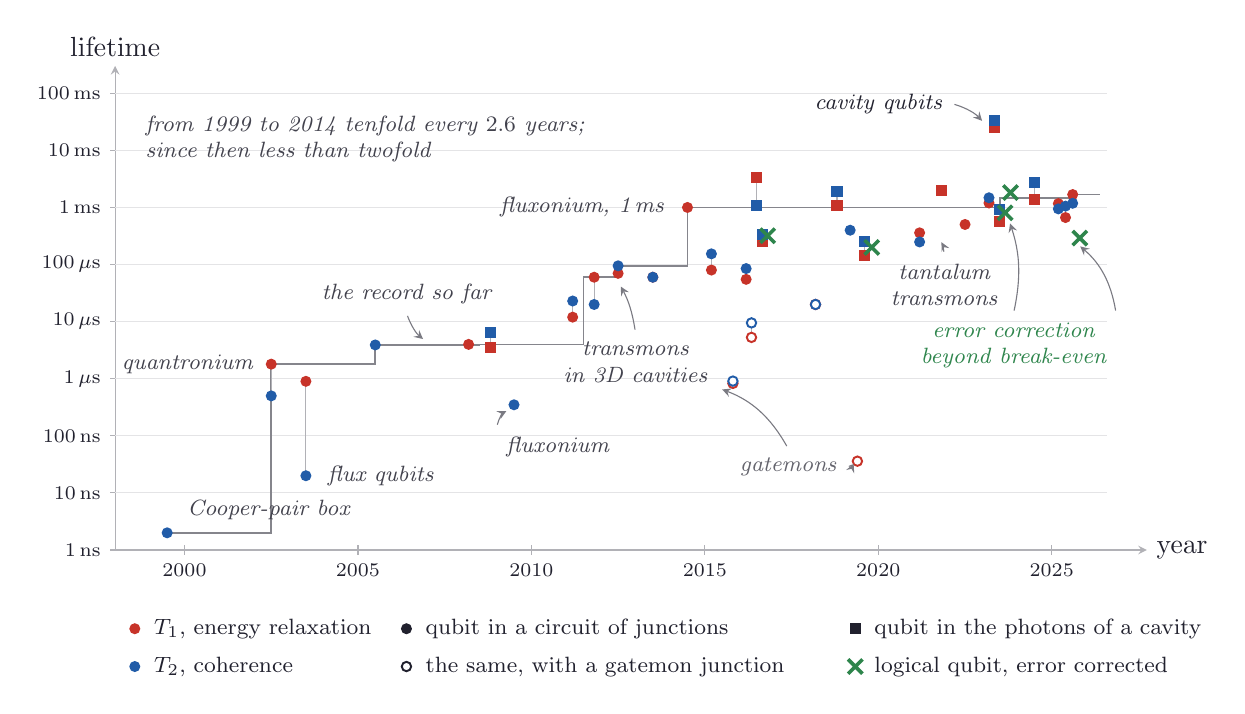
\begin{tikzpicture}[ink/.style={line width=0.9pt, ndInk}, faint/.style={line width=0.4pt, ndInk!35}, dashedink/.style={line width=0.5pt, ndInk!55, dash pattern=on 2.5pt off 2pt}, vec/.style={->, >=stealth, line width=1.2pt}, note/.style={font=\footnotesize\itshape, text=ndInk!85, align=center}, pointer/.style={->, >=stealth, line width=0.4pt, ndInk!60, shorten >=2pt, shorten <=1pt}, dot/.style={circle, fill=ndInk, inner sep=0pt, minimum size=3.4pt}, wash/.style={fill=ndSky, fill opacity=0.55}, every node/.style={text=ndInk}]
\definecolor{ndInk}{rgb}{0.13,0.13,0.18}
\definecolor{ndPaper}{rgb}{0.99,0.96,0.88}
\definecolor{ndSky}{rgb}{0.84,0.91,0.98}
\definecolor{ndRose}{rgb}{0.98,0.86,0.84}
\definecolor{ndBlue}{rgb}{0.13,0.36,0.66}
\definecolor{ndRed}{rgb}{0.78,0.20,0.16}
\definecolor{ndGold}{rgb}{0.88,0.62,0.10}
\definecolor{ndGreen}{rgb}{0.18,0.52,0.30}
\draw[faint, ->, >=stealth] (0.000,0.000) -- (13.104,0.000) node[right, text=ndInk] {year};
\draw[faint, ->, >=stealth] (0.000,0.000) -- (0.000,6.148) node[above, text=ndInk] {lifetime};
\draw[faint] (0.881,0.060) -- (0.881,-0.060) node[below, font=\scriptsize, text=ndInk] {$2000$};
\draw[faint] (3.084,0.060) -- (3.084,-0.060) node[below, font=\scriptsize, text=ndInk] {$2005$};
\draw[faint] (5.287,0.060) -- (5.287,-0.060) node[below, font=\scriptsize, text=ndInk] {$2010$};
\draw[faint] (7.490,0.060) -- (7.490,-0.060) node[below, font=\scriptsize, text=ndInk] {$2015$};
\draw[faint] (9.692,0.060) -- (9.692,-0.060) node[below, font=\scriptsize, text=ndInk] {$2020$};
\draw[faint] (11.895,0.060) -- (11.895,-0.060) node[below, font=\scriptsize, text=ndInk] {$2025$};
\draw[faint] (0.060,0.000) -- (-0.060,0.000) node[left, font=\scriptsize, text=ndInk] {1\,ns};
\draw[faint] (0.060,0.725) -- (-0.060,0.725) node[left, font=\scriptsize, text=ndInk] {10\,ns};
\draw[faint] (0.060,1.450) -- (-0.060,1.450) node[left, font=\scriptsize, text=ndInk] {100\,ns};
\draw[faint] (0.060,2.175) -- (-0.060,2.175) node[left, font=\scriptsize, text=ndInk] {1\,$\mu$s};
\draw[faint] (0.060,2.900) -- (-0.060,2.900) node[left, font=\scriptsize, text=ndInk] {10\,$\mu$s};
\draw[faint] (0.060,3.625) -- (-0.060,3.625) node[left, font=\scriptsize, text=ndInk] {100\,$\mu$s};
\draw[faint] (0.060,4.350) -- (-0.060,4.350) node[left, font=\scriptsize, text=ndInk] {1\,ms};
\draw[faint] (0.060,5.075) -- (-0.060,5.075) node[left, font=\scriptsize, text=ndInk] {10\,ms};
\draw[faint] (0.060,5.800) -- (-0.060,5.800) node[left, font=\scriptsize, text=ndInk] {100\,ms};
\draw[faint, ndInk!12] (0.000,0.725) -- (12.600,0.725);
\draw[faint, ndInk!12] (0.000,1.450) -- (12.600,1.450);
\draw[faint, ndInk!12] (0.000,2.175) -- (12.600,2.175);
\draw[faint, ndInk!12] (0.000,2.900) -- (12.600,2.900);
\draw[faint, ndInk!12] (0.000,3.625) -- (12.600,3.625);
\draw[faint, ndInk!12] (0.000,4.350) -- (12.600,4.350);
\draw[faint, ndInk!12] (0.000,5.075) -- (12.600,5.075);
\draw[faint, ndInk!12] (0.000,5.800) -- (12.600,5.800);
\draw[line width=0.6pt, ndInk!55] (0.661,0.218) -- (1.983,0.218) -- (1.983,2.360) -- (3.304,2.360) -- (3.304,2.604) -- (4.626,2.604) -- (4.626,2.611) -- (5.948,2.611) -- (5.948,3.162) -- (5.948,3.162) -- (5.948,3.464) -- (6.388,3.464) -- (6.388,3.609) -- (7.269,3.609) -- (7.269,4.350) -- (11.234,4.350) -- (11.234,4.473) -- (12.115,4.473) -- (12.115,4.514) -- (12.512,4.514);
\fill[ndBlue] (0.661,0.218) circle (2.0pt);
\draw[faint] (1.983,2.360) -- (1.983,1.957);
\fill[ndRed] (1.983,2.360) circle (2.0pt);
\fill[ndBlue] (1.983,1.957) circle (2.0pt);
\draw[faint] (2.423,2.142) -- (2.423,0.943);
\fill[ndRed] (2.423,2.142) circle (2.0pt);
\fill[ndBlue] (2.423,0.943) circle (2.0pt);
\fill[ndBlue] (3.304,2.604) circle (2.0pt);
\fill[ndRed] (4.489,2.611) circle (2.0pt);
\fill[ndBlue] (5.066,1.844) circle (2.0pt);
\draw[faint] (5.811,2.957) -- (5.811,3.162);
\fill[ndRed] (5.811,2.957) circle (2.0pt);
\fill[ndBlue] (5.811,3.162) circle (2.0pt);
\draw[faint] (6.084,3.464) -- (6.084,3.118);
\fill[ndRed] (6.084,3.464) circle (2.0pt);
\fill[ndBlue] (6.084,3.118) circle (2.0pt);
\draw[faint] (6.388,3.513) -- (6.388,3.609);
\fill[ndRed] (6.388,3.513) circle (2.0pt);
\fill[ndBlue] (6.388,3.609) circle (2.0pt);
\draw[faint] (6.829,3.464) -- (6.829,3.464);
\fill[ndRed] (6.829,3.464) circle (2.0pt);
\fill[ndBlue] (6.829,3.464) circle (2.0pt);
\fill[ndRed] (7.269,4.350) circle (2.0pt);
\draw[faint] (7.573,3.555) -- (7.573,3.761);
\fill[ndRed] (7.573,3.555) circle (2.0pt);
\fill[ndBlue] (7.573,3.761) circle (2.0pt);
\draw[faint] (8.014,3.437) -- (8.014,3.574);
\fill[ndRed] (8.014,3.437) circle (2.0pt);
\fill[ndBlue] (8.014,3.574) circle (2.0pt);
\fill[ndBlue] (9.335,4.061) circle (2.0pt);
\draw[faint] (10.217,4.028) -- (10.217,3.912);
\fill[ndRed] (10.217,4.028) circle (2.0pt);
\fill[ndBlue] (10.217,3.912) circle (2.0pt);
\fill[ndRed] (10.794,4.134) circle (2.0pt);
\draw[faint] (11.098,4.407) -- (11.098,4.473);
\fill[ndRed] (11.098,4.407) circle (2.0pt);
\fill[ndBlue] (11.098,4.473) circle (2.0pt);
\draw[faint] (11.979,4.399) -- (11.979,4.332);
\fill[ndRed] (11.979,4.399) circle (2.0pt);
\fill[ndBlue] (11.979,4.332) circle (2.0pt);
\draw[faint] (12.070,4.222) -- (12.070,4.367);
\fill[ndRed] (12.070,4.222) circle (2.0pt);
\fill[ndBlue] (12.070,4.367) circle (2.0pt);
\draw[faint] (12.161,4.514) -- (12.161,4.403);
\fill[ndRed] (12.161,4.514) circle (2.0pt);
\fill[ndBlue] (12.161,4.403) circle (2.0pt);
\draw[faint] (7.846,2.116) -- (7.846,2.145);
\draw[ndRed, line width=0.7pt, fill=white] (7.846,2.116) circle (1.7pt);
\draw[ndBlue, line width=0.7pt, fill=white] (7.846,2.145) circle (1.7pt);
\draw[faint] (8.082,2.700) -- (8.082,2.884);
\draw[ndRed, line width=0.7pt, fill=white] (8.082,2.700) circle (1.7pt);
\draw[ndBlue, line width=0.7pt, fill=white] (8.082,2.884) circle (1.7pt);
\draw[faint] (8.895,3.118) -- (8.895,3.118);
\draw[ndRed, line width=0.7pt, fill=white] (8.895,3.118) circle (1.7pt);
\draw[ndBlue, line width=0.7pt, fill=white] (8.895,3.118) circle (1.7pt);
\draw[ndRed, line width=0.7pt, fill=white] (9.427,1.128) circle (1.7pt);
\draw[faint] (4.762,2.567) -- (4.762,2.766);
\fill[ndRed] (4.762,2.567) ++(-2.0pt,-2.0pt) rectangle ++(4.0pt,4.0pt);
\fill[ndBlue] (4.762,2.766) ++(-2.0pt,-2.0pt) rectangle ++(4.0pt,4.0pt);
\draw[faint] (8.150,4.726) -- (8.150,4.380);
\fill[ndRed] (8.150,4.726) ++(-2.0pt,-2.0pt) rectangle ++(4.0pt,4.0pt);
\fill[ndBlue] (8.150,4.380) ++(-2.0pt,-2.0pt) rectangle ++(4.0pt,4.0pt);
\draw[faint] (8.219,3.914) -- (8.219,4.001);
\fill[ndRed] (8.219,3.914) ++(-2.0pt,-2.0pt) rectangle ++(4.0pt,4.0pt);
\fill[ndBlue] (8.219,4.001) ++(-2.0pt,-2.0pt) rectangle ++(4.0pt,4.0pt);
\draw[faint] (9.168,4.380) -- (9.168,4.552);
\fill[ndRed] (9.168,4.380) ++(-2.0pt,-2.0pt) rectangle ++(4.0pt,4.0pt);
\fill[ndBlue] (9.168,4.552) ++(-2.0pt,-2.0pt) rectangle ++(4.0pt,4.0pt);
\draw[faint] (9.518,3.738) -- (9.518,3.916);
\fill[ndRed] (9.518,3.738) ++(-2.0pt,-2.0pt) rectangle ++(4.0pt,4.0pt);
\fill[ndBlue] (9.518,3.916) ++(-2.0pt,-2.0pt) rectangle ++(4.0pt,4.0pt);
\fill[ndRed] (10.490,4.568) ++(-2.0pt,-2.0pt) rectangle ++(4.0pt,4.0pt);
\draw[faint] (11.166,5.371) -- (11.166,5.460);
\fill[ndRed] (11.166,5.371) ++(-2.0pt,-2.0pt) rectangle ++(4.0pt,4.0pt);
\fill[ndBlue] (11.166,5.460) ++(-2.0pt,-2.0pt) rectangle ++(4.0pt,4.0pt);
\draw[faint] (11.234,4.177) -- (11.234,4.322);
\fill[ndRed] (11.234,4.177) ++(-2.0pt,-2.0pt) rectangle ++(4.0pt,4.0pt);
\fill[ndBlue] (11.234,4.322) ++(-2.0pt,-2.0pt) rectangle ++(4.0pt,4.0pt);
\draw[faint] (11.675,4.456) -- (11.675,4.663);
\fill[ndRed] (11.675,4.456) ++(-2.0pt,-2.0pt) rectangle ++(4.0pt,4.0pt);
\fill[ndBlue] (11.675,4.663) ++(-2.0pt,-2.0pt) rectangle ++(4.0pt,4.0pt);
\draw[ndGreen, line width=1.3pt] (8.287,3.991) ++(-2.6pt,-2.6pt) -- ++(5.2pt,5.2pt) ++(-5.2pt,0) -- ++(5.2pt,-5.2pt);
\draw[ndGreen, line width=1.3pt] (9.609,3.843) ++(-2.6pt,-2.6pt) -- ++(5.2pt,5.2pt) ++(-5.2pt,0) -- ++(5.2pt,-5.2pt);
\draw[ndGreen, line width=1.3pt] (11.303,4.282) ++(-2.6pt,-2.6pt) -- ++(5.2pt,5.2pt) ++(-5.2pt,0) -- ++(5.2pt,-5.2pt);
\draw[ndGreen, line width=1.3pt] (11.371,4.539) ++(-2.6pt,-2.6pt) -- ++(5.2pt,5.2pt) ++(-5.2pt,0) -- ++(5.2pt,-5.2pt);
\draw[ndGreen, line width=1.3pt] (12.252,3.961) ++(-2.6pt,-2.6pt) -- ++(5.2pt,5.2pt) ++(-5.2pt,0) -- ++(5.2pt,-5.2pt);
\begin{scope}[shift={(0.250,-1.000)}]\fill[ndRed] (0,0) circle (2.0pt);\end{scope}
\node[anchor=west, font=\footnotesize] at (0.370,-1.000) {$T_1$, energy relaxation};
\begin{scope}[shift={(3.700,-1.000)}]\fill[ndInk] (0,0) circle (2.0pt);\end{scope}
\node[anchor=west, font=\footnotesize] at (3.820,-1.000) {qubit in a circuit of junctions};
\begin{scope}[shift={(9.400,-1.000)}]\fill[ndInk] (-2.0pt,-2.0pt) rectangle (2.0pt,2.0pt);\end{scope}
\node[anchor=west, font=\footnotesize] at (9.520,-1.000) {qubit in the photons of a cavity};
\begin{scope}[shift={(0.250,-1.480)}]\fill[ndBlue] (0,0) circle (2.0pt);\end{scope}
\node[anchor=west, font=\footnotesize] at (0.370,-1.480) {$T_2$, coherence};
\begin{scope}[shift={(3.700,-1.480)}]\draw[ndInk, line width=0.7pt] (0,0) circle (1.7pt);\end{scope}
\node[anchor=west, font=\footnotesize] at (3.820,-1.480) {the same, with a gatemon junction};
\begin{scope}[shift={(9.400,-1.480)}]\draw[ndGreen, line width=1.3pt] (-2.6pt,-2.6pt) -- (2.6pt,2.6pt) (-2.6pt,2.6pt) -- (2.6pt,-2.6pt);\end{scope}
\node[anchor=west, font=\footnotesize] at (9.520,-1.480) {logical qubit, error corrected};
\node[note, anchor=south west] at (0.793,0.262) {Cooper-pair box};
\node[note, anchor=east] at (1.872,2.360) {quantronium};
\node[note, anchor=west] at (2.577,0.943) {flux qubits};
\node[note, anchor=north west] (fl) at (4.846,1.556) {fluxonium};
\draw[pointer] (fl.north west) to[bend left=25] (5.031,1.796);
\node[note, anchor=north, text=ndInk!70] (gm) at (8.547,1.289) {gatemons};
\draw[pointer] (gm.north) to[bend right=20] (7.644,2.063);
\draw[pointer] (gm.east) to[bend right=25] (9.406,1.161);
\node[note, anchor=north] (tr) at (6.608,2.764) {transmons\\ in 3D cavities};
\draw[pointer] (tr.north) to[bend right=10] (6.388,3.407);
\node[note, anchor=north] (ta) at (10.529,3.753) {tantalum\\ transmons};
\draw[pointer] (ta.north) to[bend right=10] (10.463,3.971);
\node[note, anchor=south, text=ndInk] (cv) at (9.692,5.421) {cavity qubits};
\draw[pointer] (cv.east) to[bend left=15] (11.058,5.399);
\node[note, anchor=north, text=ndGreen] (qe) at (11.410,3.006) {error correction\\ beyond break-even};
\draw[pointer] (qe.north) to[bend right=15] (11.344,4.214);
\draw[pointer] (qe.north east) to[bend right=20] (12.203,3.901);
\node[note, anchor=south] (rc) at (3.701,3.006) {the record so far};
\draw[pointer] (rc.south) to[bend right=15] (3.965,2.634);
\node[note, anchor=east] at (7.093,4.350) {fluxonium, 1\,ms};
\node[note, anchor=north west, align=left] at (0.264,5.639) {from 1999 to 2014 tenfold every $2.6$ years;\\ since then less than twofold};
\end{tikzpicture}
